\subsection{External Interface Requirements}
Here is shown the mockups of the UI. With the exception of the home page, which is shown from both the guest’s and the user’s perspectives, all other screens are displayed only from the user’s perspective, since the only differences are already shown on the home page.
\vspace{3mm}
\newline
\textbf{Home page} \newline
The \emph{Home page} acts as a dashboard for exploration. It assumes the cyclist immediately wants to either find a safe path to ride or start recording their own journey. On the left, the home page is shown from the user’s perspective; on the right, from the guest’s perspective

\begin{figure}[H]
    \centering
    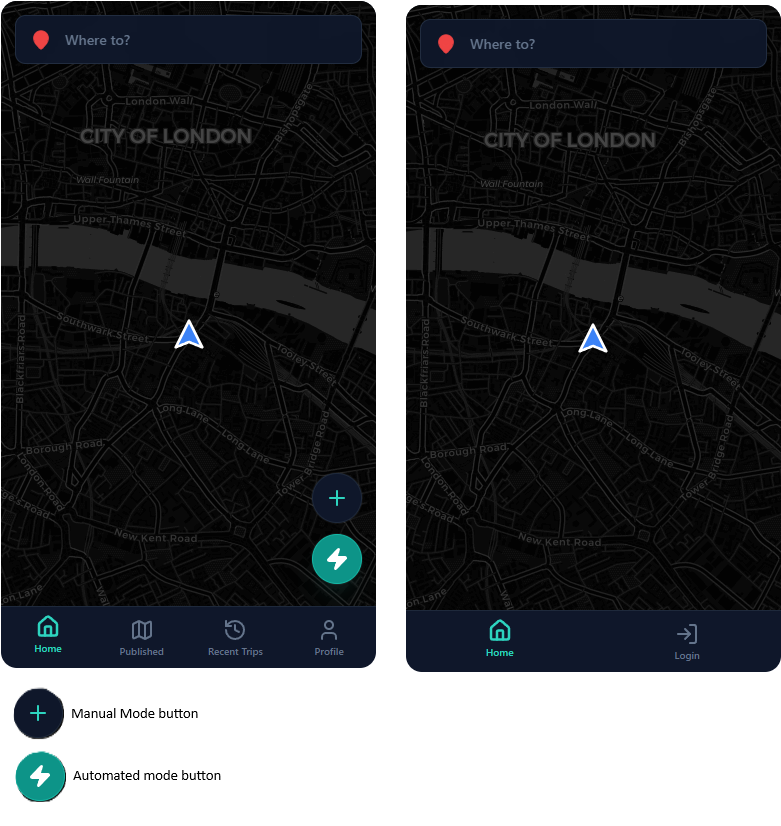
\includegraphics[width=1\linewidth]{RASD/Images/Mockup/HomePage.png}
    \caption{Home page}
    \label{fig:placeholder}
\end{figure}

\newpage
\noindent
\textbf{Search path} \newline
From the \emph{Home page}, when the cyclist inserts a destination, the five paths that connect origin and destination with the highest score will appear on the map. If the cyclist wants to change the origin to a location that is not the current location, the “Start Navigation” button will disappear.

\begin{figure}[H]
    \centering
    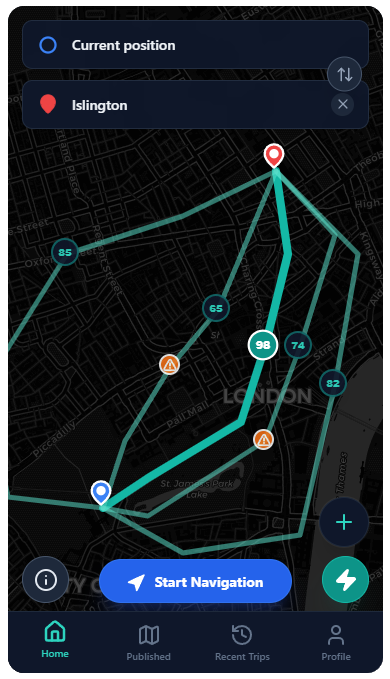
\includegraphics[width=0.6\linewidth]{RASD/Images/Mockup/StartNavigation.png}
    \caption{Start navigation screen}
    \label{fig:placeholder}
\end{figure}

\newpage
\noindent
\textbf{Navigation} \newline
From the \emph{Search path screen}, when the cyclist clicks “Start Navigation”, the navigation begin and the \emph{Navigation sreen} appears. When the cyclist reaches the destination, the navigation ends and the \emph{Trip completed screen} appears.

\begin{figure}[h!]
    \centering
    \subfloat[Navigation screen]{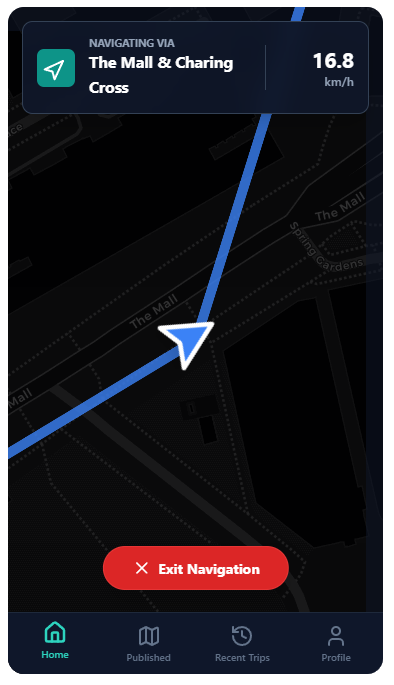
\includegraphics[width=0.5\textwidth]{RASD/Images/Mockup/Navigation.png}}\hfill
    \subfloat[Trip completed screen]{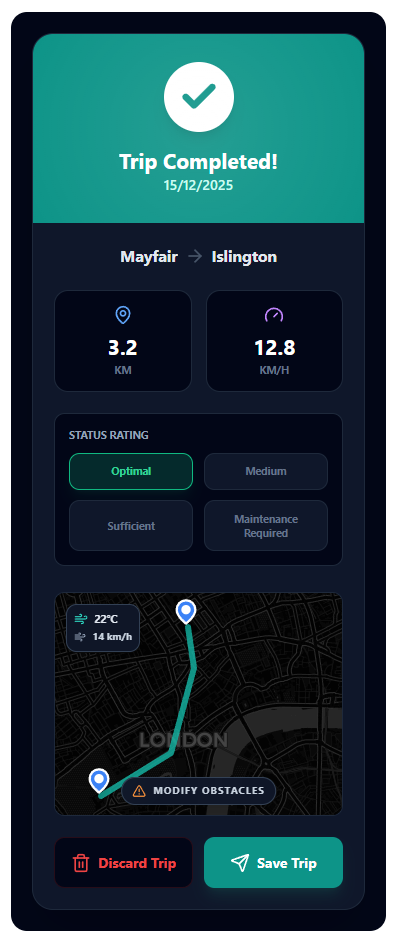
\includegraphics[width=0.5\textwidth]{RASD/Images/Mockup/NavigationCompleted.png}}
\end{figure}

\newpage
\noindent
\textbf{Manual Mode} \newline
From the \emph{Home page}, when the user clicks the “Manual Mode” button, the \emph{Draw Path screen} appears. Here, the user can draw a path by clicking on the map to add points, which the Map Service then connects to create a path that follows the street layout. By clicking “Obstacles”, the \emph{Insert Obstacles screen} appears, allowing the user to place obstacles directly on the map. Finally, clicking “Next Step” opens the \emph{Review \& Publish screen}, where the user sets the status and publishes the path by clicking “Publish Path”.
\begin{figure}[h!]
    \centering
    \subfloat[Draw path screen]{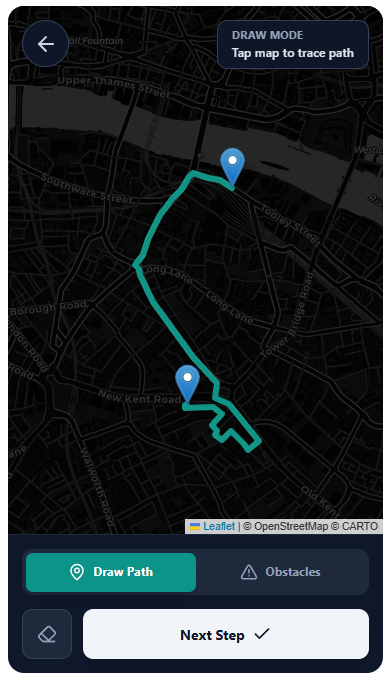
\includegraphics[width=0.33\textwidth]{RASD/Images/Mockup/DrawPath.png}}\hfill
    \subfloat[Insert obstacles screen]{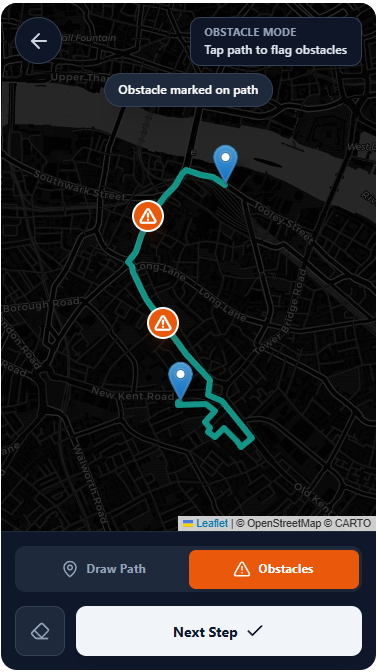
\includegraphics[width=0.33\textwidth]{RASD/Images/Mockup/InsertObstacles.png}}
    \subfloat[Review \& publish screen]{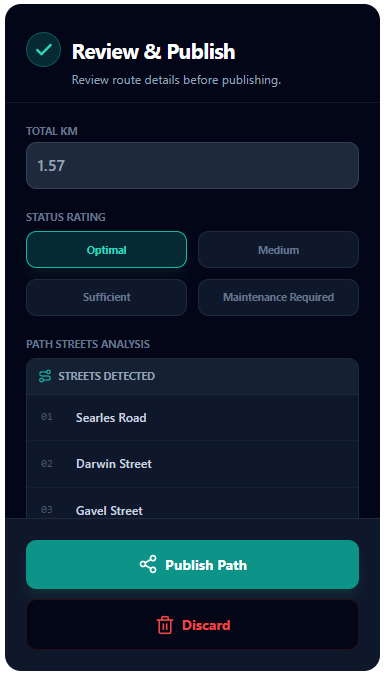
\includegraphics[width=0.33\textwidth]{RASD/Images/Mockup/Review&Publish.png}}
\end{figure}

\newpage
\noindent

\newpage
\subsection{Functional Requirements}

\textbf{Sign up \& Login}
\begin{description}
    \item[\textbf{[R1]}] The platform shall allow new users to register an account by providing personal information.
    \item[\textbf{[R2]}] The platform shall allow registered users to log in by entering their registered email and password.
\end{description}

\noindent
\textbf{Map Explorer}
\begin{description}
    \item[\textbf{[R3]}] The platform shall display an interactive map centered on the user's current location.
    \item[\textbf{[R4]}] The platform shall allow users to input an "Origin" and "Destination" of the desired path.
    \item[\textbf{[R5]}] The platform shall allow users to swap the origin and destination inputs.
    \item[\textbf{[R6]}] The platform shall calculate and display the top 5 paths options ranked by score.
    \item[\textbf{[R7]}] The platform shall visualize the geometry, quality, scores and obstacles of the top 5 paths on the map.
    \item[\textbf{[R8]}] The platform shall allow users to start the navigation mode for the currently selected path.
    \item[\textbf{[R9]}] When the navigation is started, the platform shall visualize the user's position in real-time.
    \item[\textbf{[R10]}] When the navigation is started, the platform shall display a dynamic navigation overlay providing the name of the street being traversed and the estimated speed.

    \item[\textbf{[R11]}] the platform shall allow users to interrupt the active navigation mode at any time.

    \item[\textbf{[R12]}]  When the navigation is completed, the platform shall present to registered users a summary screen containing statistics and the map of the path taken.

    \item[\textbf{[R13]}] When the navigation is completed, the platform shall allow registered users to modify the path status and the obstacles.
\end{description}

\noindent
\textbf{Active Path Recording}
\begin{description}
    \item[\textbf{[R14]}] The platform shall allow registered users to start an active recording session.
    \item[\textbf{[R15]}] The platform shall allow registered users to pause and resume the recording of the active trip.
    \item[\textbf{[R16]}] The platform shall utilize device sensors to automatically detect obstacles.
    \item[\textbf{[R17]}] The platform shall display real-time metrics during the trip, including duration, current speed, distance traveled, and weather conditions.

    \item[\textbf{[R18]}] The platform shall allow registered users to stop the recording and immediately transition to the summary screen to review the captured data.

    \item[\textbf{[R19]}] The platform shall allow registered users to modify status and obstacles in the captured data summary.

    \item[\textbf{[R20]}] The platform shall allow registered users to publish the captured path along with its data.
\end{description}

\newpage
\noindent
\textbf{Manual Path Creation}
\begin{description}
    \item[\textbf{[R21]}] The platform shall allow registered users to manually draw the path on the map.
    \item[\textbf{[R22]}] The platform shall allow registered users to manually place obstacle markers along the drawn path.
    \item[\textbf{[R23]}] The platform shall allow registered users to set the status of the drawn path.
    \item[\textbf{[R24]}] The platform shall allow registered users to publish the drawn path along with its data.
\end{description}

\noindent
\textbf{Trips \& Published Paths}
\begin{description}
    \item[\textbf{[R25]}] The platform shall display a dashboard listing the user's historical trips and their data, sorted chronologically.
    \item[\textbf{[R26]}] The platform shall allow registered users to view a list of paths published by them.
    \item[\textbf{[R27]}] The platform shall allow registered users to edit the information of any of their published paths.
    \item[\textbf{[R28]}] The platform shall allow registered users to delete any of their published paths.
\end{description}

\noindent
\textbf{User Profile}
\begin{description}
    \item[\textbf{[R29]}] The platform shall display a user profile screen summarizing the main aggregate statistics.
    \item[\textbf{[R30]}] The platform shall allow registered users to edit their profile information.
\end{description}



\newpage
\subsubsection{Use Cases Diagrams}
    \begin{figure}[H]
        \centering
        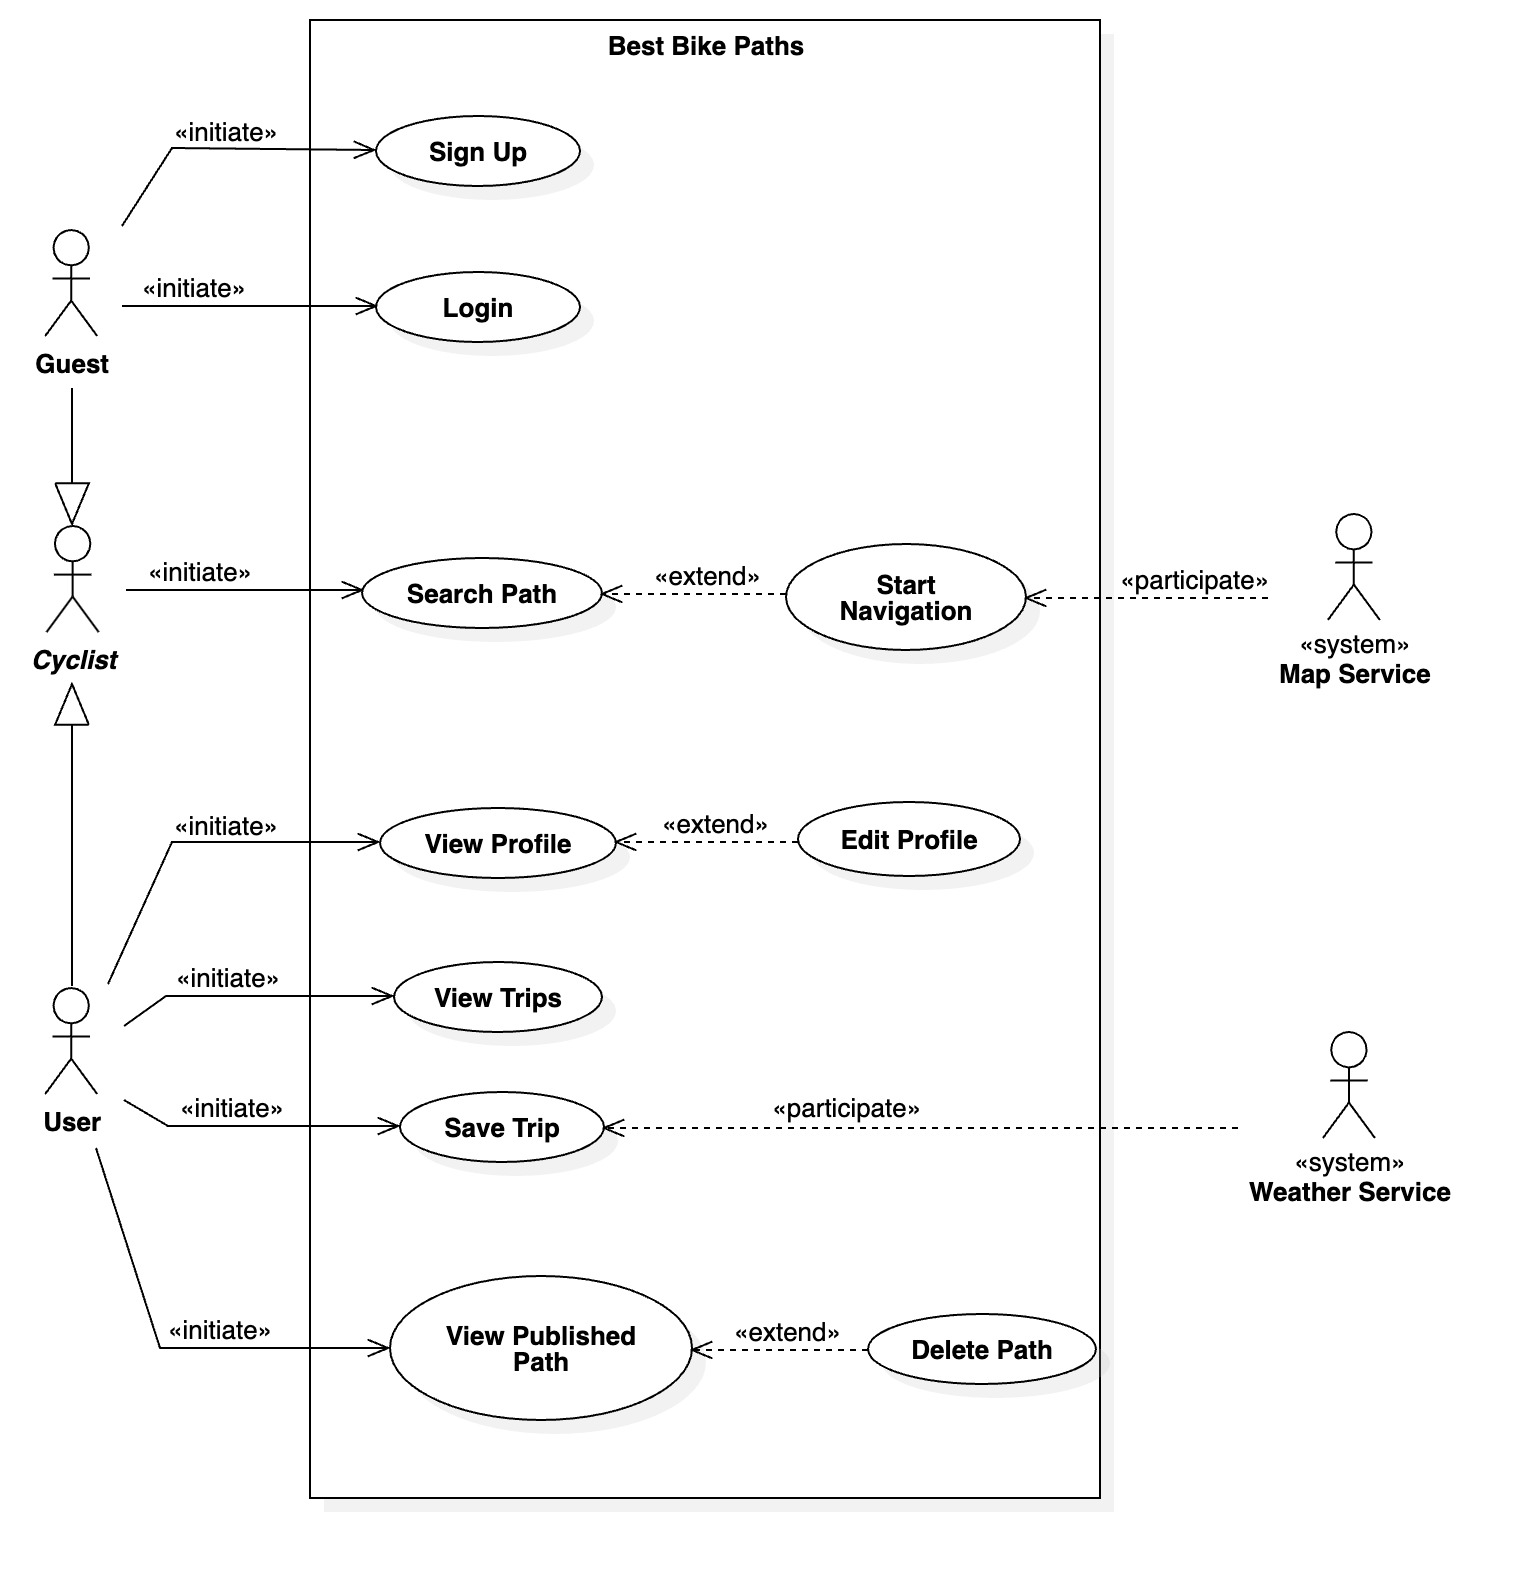
\includegraphics[width=1\linewidth]{RASD/Images/UseCaseDiagrams/GuestCyclistUser.jpg}
        \caption{General Utilities Use Case Diagram}
        \label{fig:placeholder}
    \end{figure}

This Use Case Diagram depicts the system’s functionalities organized through a generalization hierarchy. The abstract actor Cyclist represents the baseline capability of searching for paths, which is common to all users. Two actors inherit from this base:

\begin{itemize}
    \item The Guest (unauthenticated), who extends the base capability with access-control operations.
    \item The User (authenticated), who extends the base capability with the full suite of platform features.
\end{itemize}

Finally, the diagram illustrates the participation of external services (Map and Weather Services) in supporting these functionalities.
\newpage
\begin{figure}[H]
    \centering
    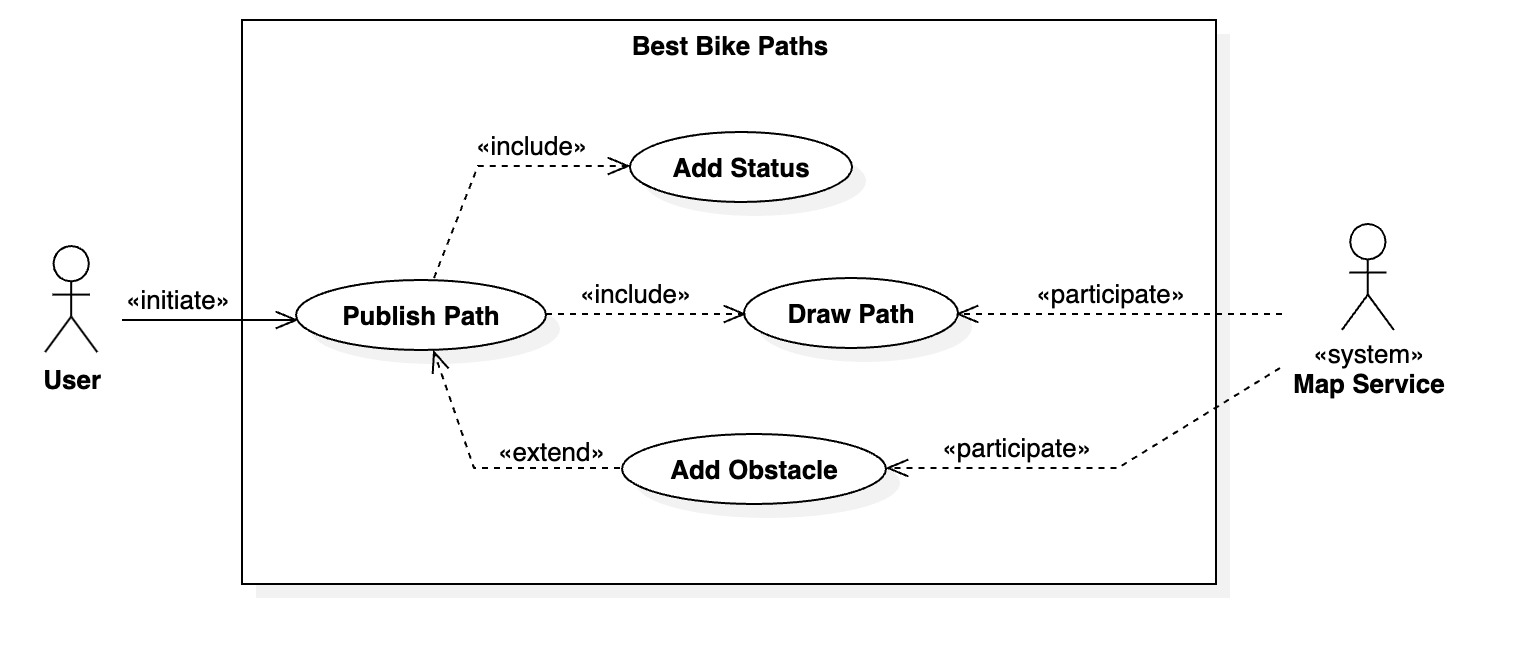
\includegraphics[width=1\linewidth]{RASD/Images/UseCaseDiagrams/ManualMode.jpg}
    \caption{Manual Mode Use Case Diagram}
    \label{fig:manual_mode}
\end{figure}

\noindent
This diagram illustrates the manual path creation process centered on the 'Publish Path' use case. This main activity mandatorily includes both 'Draw Path' (to define the route geometry) and 'Add Status' (to assign a rating). Additionally, the process can be optionally extended by 'Add Obstacle' to allow the user to report specific issues on the map.

\vspace{15mm}

\begin{figure}[H]
    \centering
    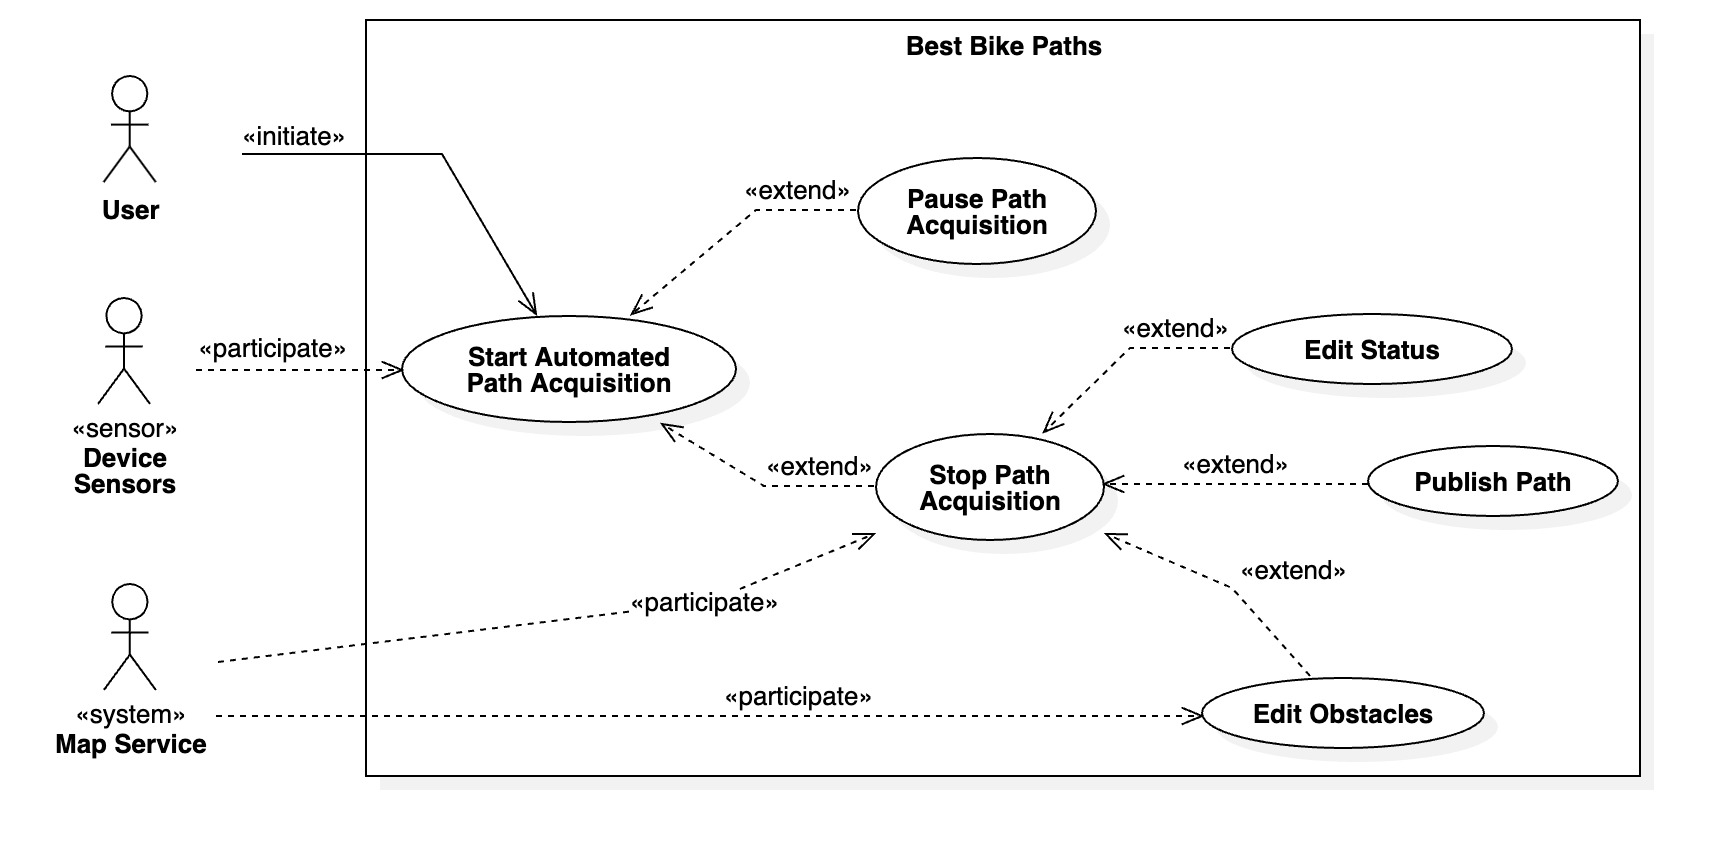
\includegraphics[width=1\linewidth]{RASD/Images/UseCaseDiagrams/AutomatedMode.jpg}
    \caption{Automated Mode Use Case Diagram}
    \label{fig:placeholder}
\end{figure}
\noindent
This diagram illustrates the automated path acquisition process. The Device Sensors actor refers to the device’s GPS, accelerometer, and gyroscope, which are essential for tracking the user's movement and detecting path quality in real-time.
\newpage

\subsubsection{Use Cases}

\setcounter{table}{0}
%tabella
\begin{table}[H]
    \centering
    \setlength\extrarowheight{2pt}
    \renewcommand{\arraystretch}{1.2}
    \begin{tabularx}{\textwidth}{|>{\bfseries}l|X|}
    \hline
    UC-01 & Sign up \\ \hline
    Actors & Guest\\ \hline
    Entry Condition &  The Guest is not currently logged in.\\ \hline
    Event Flow & 
    \begin{enumerate}
      \item The Guest opens the login screen.
      \item The Guest clicks "sign up".
      \item The Guest enters the required information.
      \item The Guest presses the "sign up" button.
      \item The platform validates the entered information.
      \item The platform sends a confirmation email to the provided email address.
      \item The platform shows a message to the guest to confirm the registration.
      \item The Guest confirms the registration by clicking on the link in the email. 
      \item The platform confirms the registration and activates the account.
      \item The Guest is redirected to the platform's homepage as a logged-in User.
    \end{enumerate}
    \\ \hline
    Exit Condition &  A new account is created and the Guest is now logged in as a User.\\ \hline
    Exception & 
    \begin{itemize}
        \item The Guest provides incorrect information.
        \item The Guest does not confirm the registration.
        \item The email is already in use.
    \end{itemize}
    \\ \hline
    \end{tabularx}
    \caption{Use Case UC-01}
    \label{UC-01}
\end{table}

\newpage
\begin{table}[H]
    \centering
    \setlength\extrarowheight{2pt}
    \renewcommand{\arraystretch}{1.2}
    \begin{tabularx}{\textwidth}{|>{\bfseries}l|X|}
    \hline
    UC-02 & Login \\ \hline
    Actors & Guest\\ \hline
    Entry Condition & The Guest is not currently logged in.\\ \hline
    Event Flow & 
    \begin{enumerate}
      \item The Guest opens the login screen.
      \item The Guest enters login credentials.
      \item The Guest clicks the "login" button.
      \item The platform verifies login credentials.
      \item The platform creates a login session for the guest.
      \item The Guest is redirected to the platform’s homepage as a logged-in User.
    \end{enumerate}
    \\ \hline
    Exit Condition & The Guest is successfully authenticated as a User.\\ \hline
    Exception & 
    \begin{itemize}
        \item The credentials provided are incorrect.
    \end{itemize}
    \\ \hline
   \end{tabularx}
   \caption{Use Case UC-02}
    \label{UC-02}
\end{table}

\begin{table}[H]
    \centering
    \setlength\extrarowheight{2pt}
    \renewcommand{\arraystretch}{1.2}
    \begin{tabularx}{\textwidth}{|>{\bfseries}l|X|}
    \hline
    UC-03 & Search Path \\ \hline
    Actors & Cyclist, Map Service\\ \hline
    Entry Condition & The Cyclist is viewing the platform’s homepage\\ \hline
    Event Flow & 
    \begin{enumerate}
      \item The platform loads the visual map from the Map Service.
      \item The Cyclist enters the origin.
      \item The Cyclist enters the destination.
      \item The platform retrieves the locations using the Map Service.
      \item The platform identifies the best 5 paths among those published.
      \item The platform displays the best 5 paths on the map.
      \item The Cyclist selects the desired path.
    \end{enumerate}
    \\ \hline
    Exit Condition &  The desired path is selected and the option to view its details is available to the Cyclist.\\ \hline
    Exception & 
    \begin{itemize}
        \item None.
    \end{itemize}
    \\ \hline
    \end{tabularx}
    \caption{Use Case UC-03}
    \label{UC-03}
\end{table} 

\begin{table}[H]
    \centering
    \setlength\extrarowheight{2pt}
    \renewcommand{\arraystretch}{1.2}
    \begin{tabularx}{\textwidth}{|>{\bfseries}l|X|}
    \hline
    UC-04 & Start Navigation \\ \hline
    Actors & Cyclist\\ \hline
    Entry Condition & The Cyclist has selected the desired path and the origin is the current location\\ \hline
    Event Flow & 
    \begin{enumerate}
      \item The platform shows the "Start Navigation" button.
      \item The Cyclist clicks "Start Navigation".
      \item The platform displays the selected path on the map.
      \item The platform guides the Cyclist in real-time.
      \item The platform detects that the Cyclist has reached the destination.
    \end{enumerate}
    \\ \hline
    Exit Condition &  The platform displays the trip summary.\\ \hline
    Exception & 
    \begin{itemize}
        \item None.
    \end{itemize}
    \\ \hline
   \end{tabularx}
   \caption{Use Case UC-04}
    \label{UC-04}
\end{table}

\begin{table}[H]
    \centering
    \setlength\extrarowheight{2pt}
    \renewcommand{\arraystretch}{1.2}
    \begin{tabularx}{\textwidth}{|>{\bfseries}l|X|}
    \hline
    UC-05 & Save trip \\ \hline
    Actors & User, Weather Service\\ \hline
    Entry Condition & The user is logged in and the navigation is completed.\\ \hline
    Event Flow & 
    \begin{enumerate}
      \item The platform retrieves weather data from the Weather Service.
      \item The platform displays the "Trip Completed" screen with statistics, weather info, and rating options. 
      \item The User selects the path status.
      \item The User clicks "Modify Obstacles" to report obstacles on the map.
      \item The User clicks "Save Trip".
      \item The platform saves the trip in the User's "Recent Trips" list.
      \item The platform automatically submits the path report to the system.
      \item The User is redirected to the "Recent Trips" screen.
    \end{enumerate}
    \\ \hline
    Exit Condition & The trip is saved and the "Recent Trips" screen is displayed to the User.\\ \hline
    Exception & 
    \begin{itemize}
        \item None.
    \end{itemize}
    \\ \hline
   \end{tabularx}
   \caption{Use Case UC-05}
    \label{UC-05}
\end{table}

\begin{table}[H]
    \centering
    \setlength\extrarowheight{2pt}
    \renewcommand{\arraystretch}{1.2}
    \begin{tabularx}{\textwidth}{|>{\bfseries}l|X|}
    \hline
    UC-06 & View Trips \\ \hline
    Actors & User\\ \hline
    Entry Condition & The User is logged in.\\ \hline
    Event Flow & 
    \begin{enumerate}
      \item The User opens the "Recent Trips" screen.
      \item The platform displays the list of saved trips.
      \item The User views the details of the trips in the list.
    \end{enumerate}
    \\ \hline
    Exit Condition &  The detailed view of the saved trips is displayed.\\ \hline
    Exception & 
    \begin{itemize}
        \item None.
    \end{itemize}
    \\ \hline
   \end{tabularx}
   \caption{Use Case UC-06}
    \label{UC-06}
\end{table}

\begin{table}[H]
    \centering
    \setlength\extrarowheight{2pt}
    \renewcommand{\arraystretch}{1.2}
    \begin{tabularx}{\textwidth}{|>{\bfseries}l|X|}
    \hline
    UC-07 & Edit Profile \\ \hline
    Actors & User\\ \hline
    Entry Condition & The User is logged in.\\ \hline
    Event Flow & 
    \begin{enumerate}
      \item The User opens the "Profile" screen.
      \item The User clicks on "Edit Profile".
      \item The User modifies the information.
      \item The User clicks "Confirm Changes"
      \item The platform validates the new data.
      \item The platform updates the profile and displays the success message.
    \end{enumerate}
    \\ \hline
    Exit Condition &  The User profile is updated with the new information.\\ \hline
    Exception & 
    \begin{itemize}
        \item The User leaves a mandatory field empty and clicks "Confirm"
    \end{itemize}
    \\ \hline
   \end{tabularx}
   \caption{Use Case UC-07}
    \label{UC-07}
\end{table}

\begin{table}[H]
    \centering
    \setlength\extrarowheight{2pt}
    \renewcommand{\arraystretch}{1.2}
    \begin{tabularx}{\textwidth}{|>{\bfseries}l|X|}
    \hline
    UC-08 & Delete path \\ \hline
    Actors & User\\ \hline
    Entry Condition & The User is logged in.\\ \hline
    Event Flow & 
    \begin{enumerate}
      \item The User opens the "Published path" screen.
      \item The User selects the path to delete.
      \item The platform displays the path details.
      \item The User clicks the "Delete" button.
      \item The platform asks for confirmation.
      \item The User confirms the deletion.
      \item The platform removes the path and updates the list.
    \end{enumerate}
    \\ \hline
    Exit Condition &  The path is permanently deleted from the published paths list.\\ \hline
    Exception & 
    \begin{itemize}
        \item None.
    \end{itemize}
    \\ \hline
   \end{tabularx}
   \caption{Use Case UC-08}
    \label{UC-08}
\end{table}

\begin{table}[H]
    \centering
    \setlength\extrarowheight{2pt}
    \renewcommand{\arraystretch}{1.2}
    \begin{tabularx}{\textwidth}{|>{\bfseries}l|X|}
    \hline
    UC-09 & Publish Path (Manual Mode) \\ \hline
    Actors & User\\ \hline
    Entry Condition & The User is logged in and is viewing the homepage.\\ \hline
    Event Flow & 
    \begin{enumerate}
      \item The User clicks the "+" button to create a new path.
      \item The platform loads the "Draw Mode" interface.
      \item The User draw the path.
      \item The User clicks the "Next Step" button.
      \item The platform displays the "Review \& Publish" screen.
      \item The User selects the status.
      \item The User clicks "Publish Path".
      \item The platform validates and makes the path available to the community.
    \end{enumerate}
    \\ \hline
    Exit Condition &  The path is published and appears in the User's "Published Paths" screen.\\ \hline
    Exception &
    \begin{itemize}
        \item  The platform detects that an identical path already exists.
    \end{itemize}
    \\ \hline
   \end{tabularx}
   \caption{Use Case UC-09}
    \label{UC-09}
\end{table}

\begin{table}[H]
    \centering
    \setlength\extrarowheight{2pt}
    \renewcommand{\arraystretch}{1.2}
    \begin{tabularx}{\textwidth}{|>{\bfseries}l|X|}
    \hline
    UC-10 & Draw Path \\ \hline
    Actors & User, Map Service\\ \hline
    Entry Condition & The User is in the 'Draw Path' mode within the manual creation interface and the interactive map is loaded.\\ \hline
    Event Flow & 
    \begin{enumerate}
      \item The User taps on the map to place the starting point.
      \item The User continues tapping to trace the path segments.
      \item The Map Service renders the route line in real-time.
      \item The platform calculates the "Total Km" dynamically.
      \item The User completes the tracing.
    \end{enumerate}
    \\ \hline
    Exit Condition &  The geometric path is defined on the map.\\ \hline
    Exception & 
    \begin{itemize}
        \item The platform fails to load the map tiles from the Map Service.
    \end{itemize}
    \\ \hline
   \end{tabularx}
   \caption{Use Case UC-10}
    \label{UC-10}
\end{table}

\begin{table}[H]
    \centering
    \setlength\extrarowheight{2pt}
    \renewcommand{\arraystretch}{1.2}
    \begin{tabularx}{\textwidth}{|>{\bfseries}l|X|}
    \hline
    UC-11 & Add Obstacle \\ \hline
    Actors & User, Map Service\\ \hline
    Entry Condition & The User is in the manual creation interface, the interactive map is loaded, and the path is partially or fully drawn.\\ \hline
    Event Flow & 
    \begin{enumerate}
      \item The User clicks on the "Obstacles" tab.
      \item The platform switches to "Obstacle Mode".
      \item The User taps a specific point along the drawn path.
      \item The platform places an obstacle marker on the coordinate using the Map Service.
    \end{enumerate}
    \\ \hline
    Exit Condition & An obstacle is flagged on the map.\\ \hline
    Exception & 
    \begin{itemize}
        \item The user adds an obstacle outside the path
    \end{itemize}
    \\ \hline
   \end{tabularx}
   \caption{Use Case UC-11}
    \label{UC-11}
\end{table}

\begin{table}[H]
    \centering
    \setlength\extrarowheight{2pt}
    \renewcommand{\arraystretch}{1.2}
    \begin{tabularx}{\textwidth}{|>{\bfseries}l|X|}
    \hline
    UC-12& Start Automated Path Acquisition \\ \hline
    Actors & User, Device Sensors\\ \hline
    Entry Condition & The User is logged in and is viewing the homepage\\ \hline
    Event Flow & 
    \begin{enumerate}
      \item The User clicks the "Lightning" button to start the acquisition.
      \item The platform initializes the "Automated Mode" interface.
      \item The platform loads the User's current location on the map using the gps from the Device Sensors.
      \item The platform starts the timer.
      \item The platform begins recording distance, speed and obstacles in real-time using the Device Sensors.
      \item The platform continuously updates the metrics (distance, obstacles, speed).
    \end{enumerate}
    \\ \hline
    Exit Condition & The path recording is active and the "Automated Mode" interface is displayed.\\ \hline
    Exception & 
    \begin{itemize}
        \item None
    \end{itemize}
    \\ \hline
   \end{tabularx}
   \caption{Use Case UC-12}
    \label{UC-12}
\end{table}

\begin{table}[H]
    \centering
    \setlength\extrarowheight{2pt}
    \renewcommand{\arraystretch}{1.2}
    \begin{tabularx}{\textwidth}{|>{\bfseries}l|X|}
    \hline
    UC-13& Pause Path Acquisition \\ \hline
    Actors & User\\ \hline
    Entry Condition & The User is logged in and the "Automated Mode" is active\\ \hline
    Event Flow & 
    \begin{enumerate}
      \item The User clicks the "Pause" button.
      \item The platform suspends the timer.
      \item The platform stops recording coordinates and metrics.
      \item The platform processes the information.
      \item The platform updates the interface to show the "Paused" state.
    \end{enumerate}
    \\ \hline
    Exit Condition & The "Automated Mode" is temporarily suspended.\\ \hline
    Exception & 
    \begin{itemize}
        \item None
    \end{itemize}
    \\ \hline
   \end{tabularx}
   \caption{Use Case UC-13}
    \label{UC-13}
\end{table}

\begin{table}[H]
    \centering
    \setlength\extrarowheight{2pt}
    \renewcommand{\arraystretch}{1.2}
    \begin{tabularx}{\textwidth}{|>{\bfseries}l|X|}
    \hline
    UC-14& Stop Path Acquisition \\ \hline
    Actors & User, Map Service\\ \hline
    Entry Condition & The User is logged in and the "Automated Mode" is active (or paused)\\ \hline
    Event Flow & 
    \begin{enumerate}
      \item The User clicks the "Stop" button.
      \item The platform stops the timer.
      \item The platform stops the data recording.
      \item The platform processes the recorded data to calculate final metrics.
      \item The platform extracts the street names using the Map Service.
      \item The platform displays the "Trip Summary" interface.
    \end{enumerate}
    \\ \hline
    Exit Condition &  The "Automated Mode" is stopped and the User is viewing the "Trip Summary"\\ \hline
    Exception & 
    \begin{itemize}
        \item None
    \end{itemize}
    \\ \hline
   \end{tabularx}
   \caption{Use Case UC-14}
    \label{UC-14}
\end{table}

\begin{table}[H]
    \centering
    \setlength\extrarowheight{2pt}
    \renewcommand{\arraystretch}{1.2}
    \begin{tabularx}{\textwidth}{|>{\bfseries}l|X|}
    \hline
    UC-15& Publish Path (Automated Mode) \\ \hline
    Actors & User\\ \hline
    Entry Condition & The User is viewing the "Trip Summary" interface with the recorded path data.\\ \hline
    Event Flow & 
    \begin{enumerate}
      \item The User clicks the "Publish Path" button.
      \item The Platform stores the path data (geometry, status, obstacles) in the system.
      \item The platform validates and makes the path available to the community..
    \end{enumerate}
    \\ \hline
    Exit Condition &  The path is published and appears in the User’s "Published Paths" screen.\\ \hline
    Exception & 
    \begin{itemize}
        \item The platform detects that an identical path already exists.
    \end{itemize}
    \\ \hline
   \end{tabularx}
   \caption{Use Case UC-15}
    \label{UC-15}
\end{table}


\newpage
\subsubsection{Sequence Diagrams}
The functions used in the sequence diagrams follow these conventional meanings:
\begin{itemize}
    \item \textbf{press(Button)}: Represents the action of a user pressing Button.
    \item \textbf{submit(Content)}: Indicates a user uploading Content to the platform.
    \item \textbf{showPage(Page)}: Displays the content of a specific Page.
    \item \textbf{showError(Error)}: Displays an error message indicating an issue that occurred.
    \item \textbf{check()}: Verifies the validity of the information provided by the user.
    \item \textbf{update(Data)}: Refers to internal processes that update database records with Data.
    \item \textbf{OpenApplication()}: Rappresent the action of a user opens the application.
    \item \textbf{getMapData()}: Represents the system requesting the visual map components from the external service.
    \item \textbf{mapTiles(Tiles)}: Delivers the graphical data required to render the map interface on the screen.
    \item \textbf{enter(Location)}: Represents the action of a user inputting a starting point or destination address.
    \item \textbf{findBestPaths(Origin, Destination)}: Identifies and returns the 5 paths with the best performance scores connecting the selected locations.
    \item \textbf{selectPath(Path)}: Represents the user choosing one of the displayed paths to view its details or start navigation.
    \item \textbf{startTracking()}: Commands the device sensors (GPS) to begin sending real-time location updates.
    \item \textbf{stopTracking()}: Commands the device sensors to cease location updates
    \item \textbf{getWeather(CurrentLocation)}: Requests meteorological data (temperature, conditions) for the specific coordinates where the trip ended.
    \item \textbf{wetherData()}: Returns the requested weather information from the external service.
    \item \textbf{insert(Object)}: Represents the user placing a marker on the map.
    \item \textbf{initializeSensors()}: Internal process that activates and configures the device's hardware to start receiving real-time data.
    \item \textbf{monitorRoadConditions()}: Analyzes data from the accelerometer and gyroscope to automatically detect potholes during the ride.
    \item \textbf{displayInstruction()}: Updates the user interface with visual navigation cues and the current position on the map.
    \item \textbf{fetchData(Criteria)}: A generic system request to retrieve specific datasets from the database required to populate or plot elements on the user interface.
    \item \textbf{showMessage(Argument)}: Shows a general message on the screen.
    \item \textbf{startTracking()}: Activates the continuous recording and initiates the loop.
    \item \textbf{monitorRoadConditions()}:Processes live sensor data to understand the path environment.
    \item \textbf{stopTracking()}: Commands the device sensors to cease location updates.

    
\end{itemize}
\newpage
\vspace{2mm}
\noindent
    \textbf{[SD1] Sign up Sequence Diagram} 
\vspace{2mm}
\begin{figure}[!h]
    \centering
    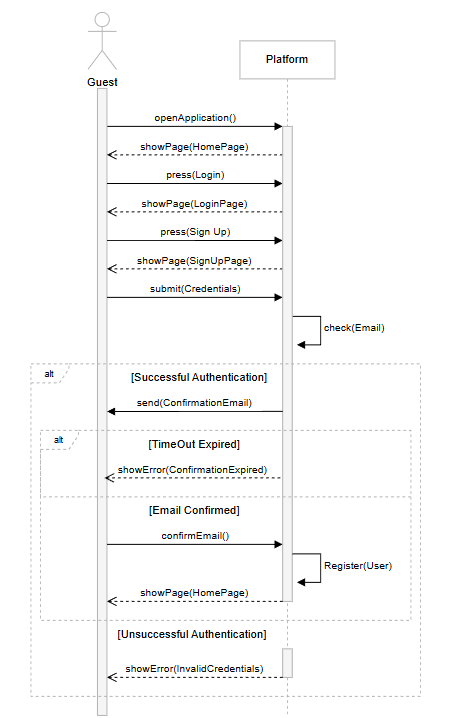
\includegraphics[width=0.8\linewidth]{RASD/Images/SEQD_SignUp.png}
    \label{fig:placeholder}
\end{figure}
\newpage
\vspace{2mm}
\noindent
    \textbf{[SD2] Login Sequence Diagram} 
\vspace{2mm}
\begin{figure}[!h]
    \centering
    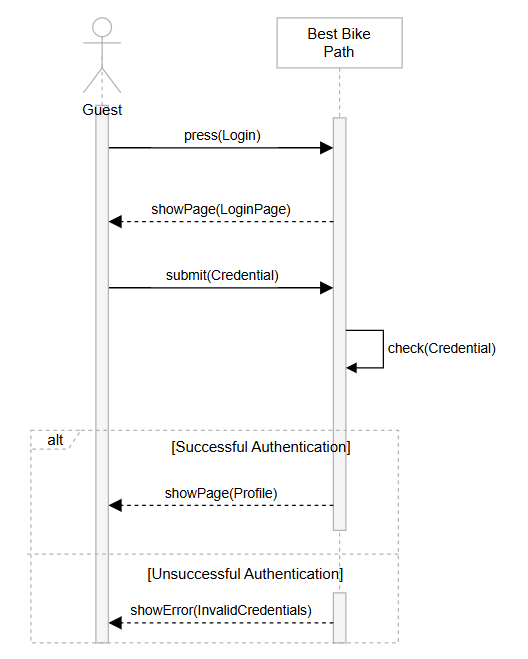
\includegraphics[width=0.8\linewidth]{RASD/Images/SEQD_Login.png}
    \label{fig:placeholder}
\end{figure}
\newpage
\vspace{2mm}
\noindent
    \textbf{[SD3] Search Path Sequence Diagram} 
\vspace{2mm}
\begin{figure}[!h]
    \centering
    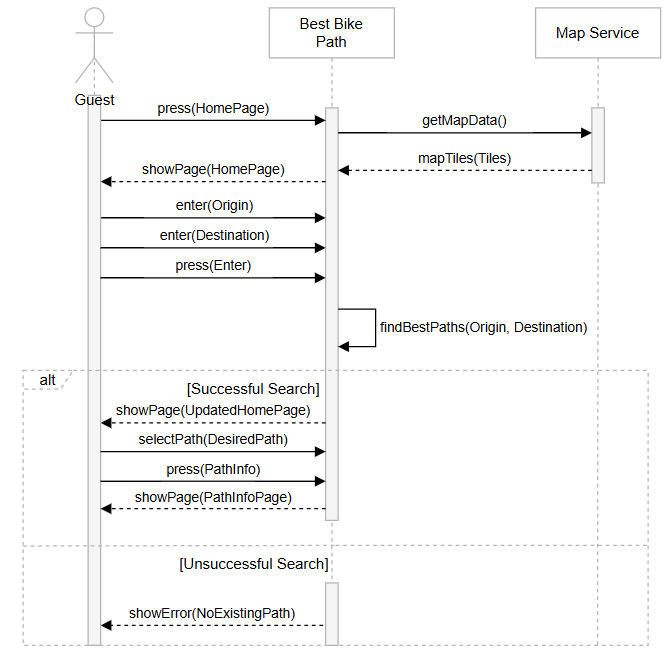
\includegraphics[width=0.8\linewidth]{RASD/Images/SEQD_search_path.png}
    \label{fig:placeholder}
\end{figure}
\newpage
\vspace{2mm}
\noindent
    \textbf{[SD4] Start Navigation Sequence Diagram} 
\vspace{2mm}
\begin{figure}[!h]
    \centering
    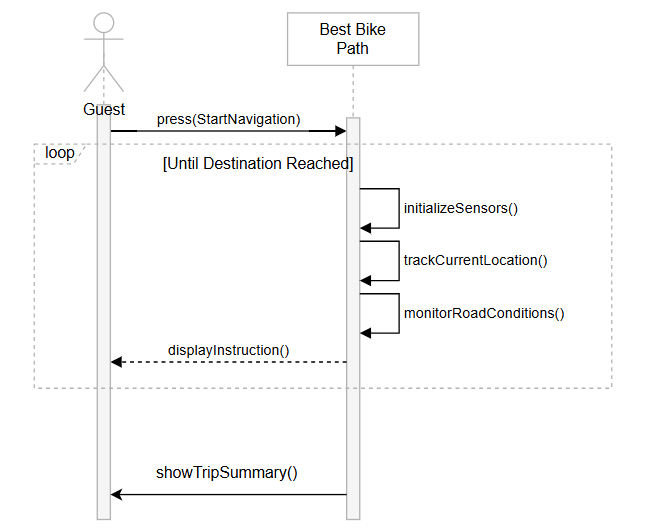
\includegraphics[width=0.8\linewidth]{RASD/Images/SEQD_start_navigation.png}
    \label{fig:placeholder}
\end{figure}
\vspace{2mm}
\newpage
\noindent
    \textbf{[SD5] Save Trip Sequence Diagram} 
\vspace{2mm}
\begin{figure}[!h]
    \centering
    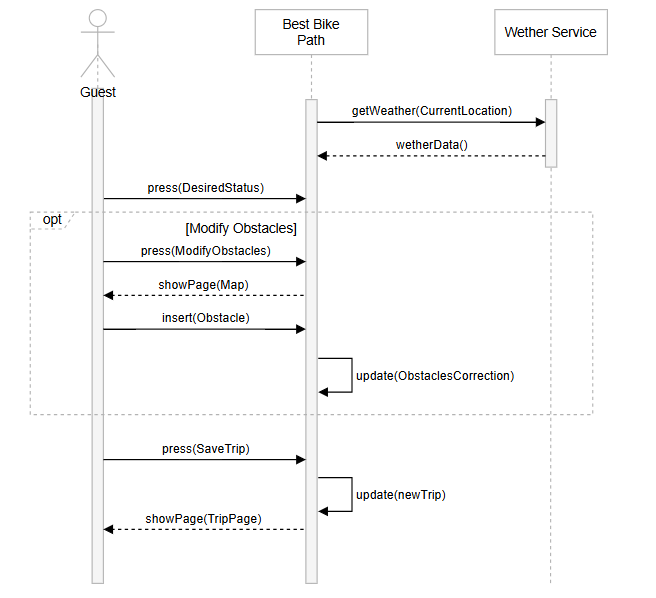
\includegraphics[width=0.8\linewidth]{RASD/Images/SEQD_save_trip.png}
    \label{fig:placeholder}
\end{figure}
\newpage
\noindent
    \textbf{[SD6] Trip View Sequence Diagram} 
\vspace{2mm}
\begin{figure}[!h]
    \centering
    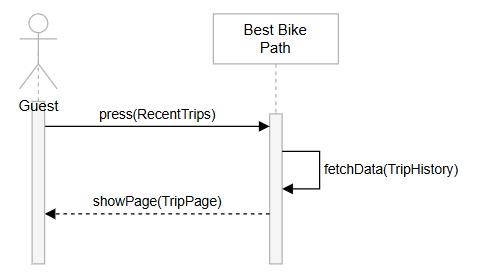
\includegraphics[width=0.8\linewidth]{RASD/Images/SEQD_view_trip.png}
    \label{fig:placeholder}
\end{figure}
\newpage
\noindent
    \textbf{[SD7] Edit Profile Sequence Diagram} 
\vspace{2mm}
\begin{figure}[!h]
    \centering
    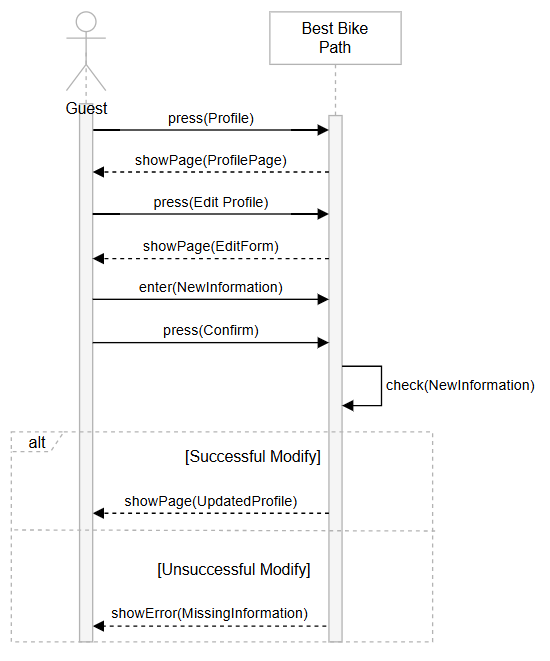
\includegraphics[width=0.8\linewidth]{RASD/Images/SEQD_edit_profile.png}
    \label{fig:placeholder}
\end{figure}
\newpage
\noindent
    \textbf{[SD8] Delete Path Sequence Diagram} 
\vspace{2mm}
\begin{figure}[!h]
    \centering
    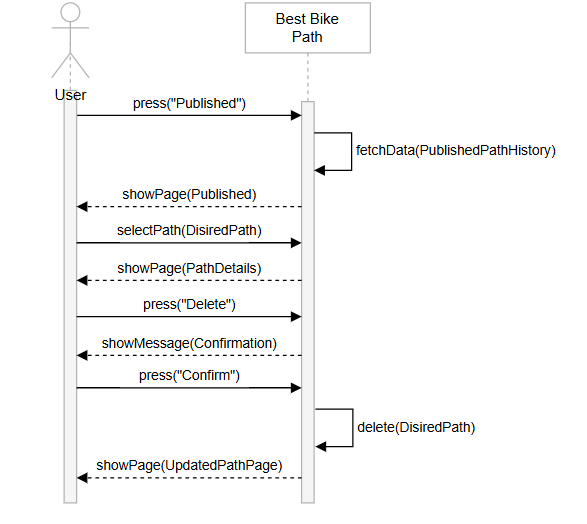
\includegraphics[width=0.8\linewidth]{RASD/Images/SEQD_delete_path.png}
    \label{fig:placeholder}
\end{figure}
\newpage
\noindent
    \textbf{[SD9] Publish Path Sequence Diagram} 
\vspace{2mm}
\begin{figure}[!h]
    \centering
    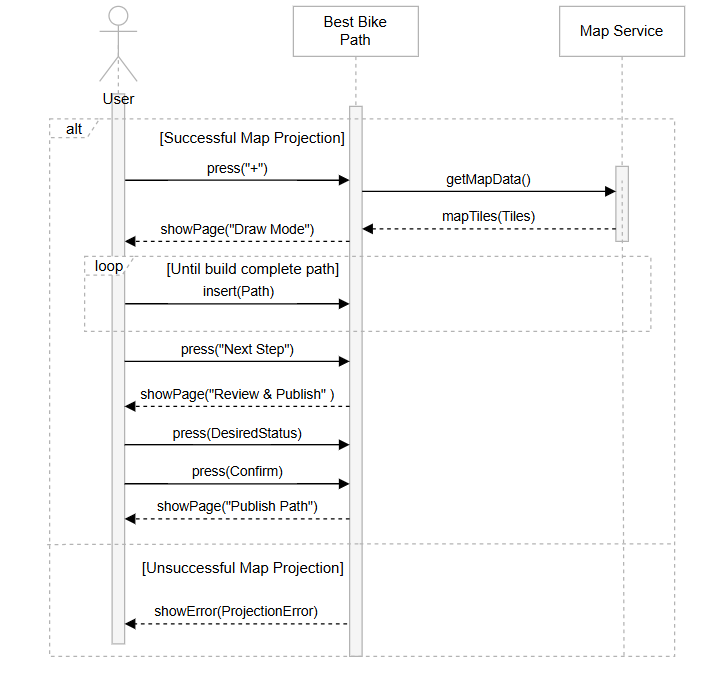
\includegraphics[width=0.8\linewidth]{RASD/Images/SEQD_publish_path_manual_mode.png}
    \label{fig:placeholder}
\end{figure}
\newpage
\noindent
    \textbf{[SD10] Draw Path Sequence Diagram} 
\vspace{2mm}
\begin{figure}[!h]
    \centering
    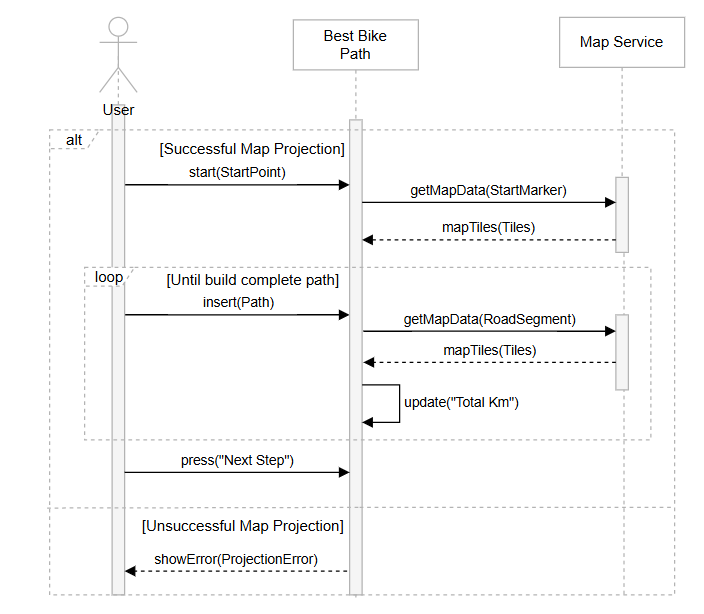
\includegraphics[width=0.8\linewidth]{RASD/Images/SEQD_draw_path.png}
    \label{fig:placeholder}
\end{figure}
\newpage
\noindent
    \textbf{[SD11] Add Obstacle Sequence Diagram} 
\vspace{2mm}
\begin{figure}[!h]
    \centering
    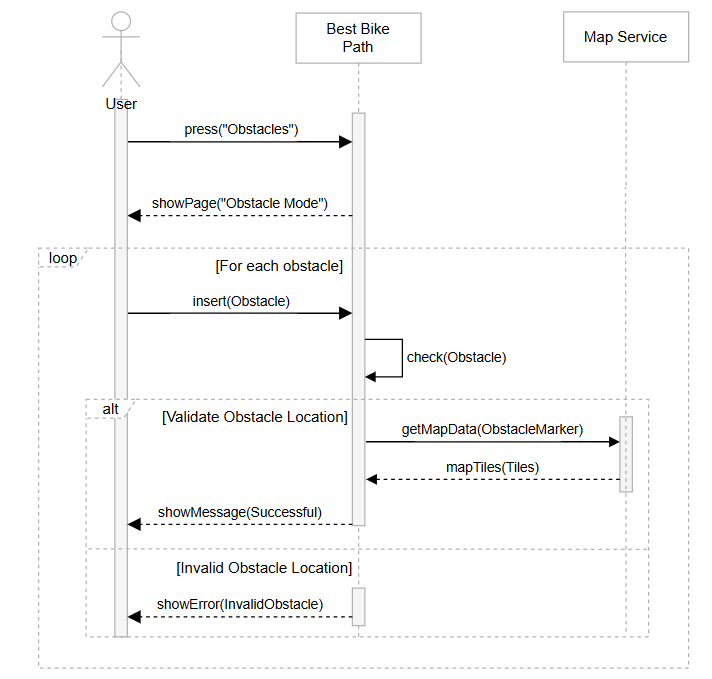
\includegraphics[width=0.8\linewidth]{RASD/Images/SEQD_add_obstacle.png}
    \label{fig:placeholder}
\end{figure}
\newpage
\noindent
    \textbf{[SD12] Start Automated Path Acquisition Sequence Diagram} 
\vspace{2mm}
\begin{figure}[!h]
    \centering
    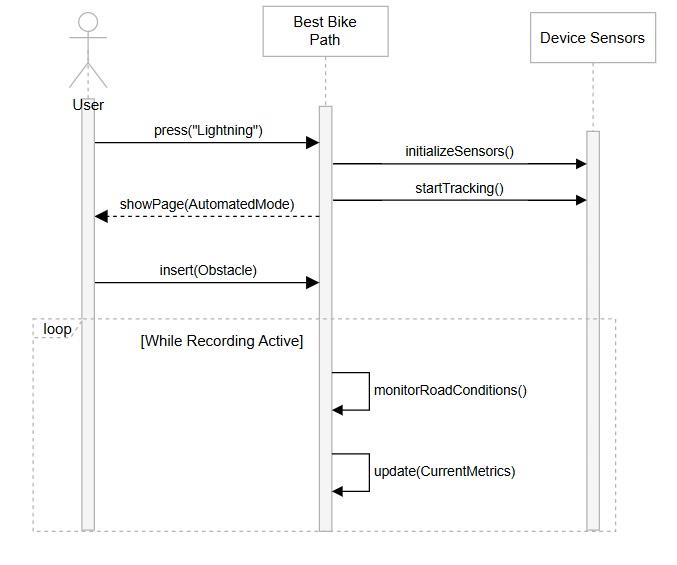
\includegraphics[width=0.8\linewidth]{RASD/Images/SEQD_start_automated_path_acquisition.png}
    \label{fig:placeholder}
\end{figure}
\newpage
\noindent
    \textbf{[SD13] Pause Path Acquisition Sequence Diagram} 
\vspace{2mm}
\begin{figure}[!h]
    \centering
    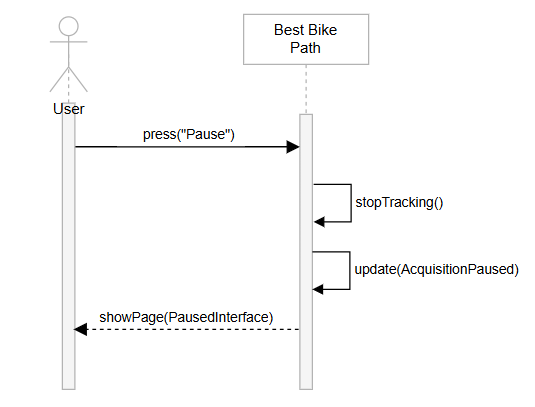
\includegraphics[width=0.8\linewidth]{RASD/Images/SEQD_pause_path_acquisition.png}
    \label{fig:placeholder}
\end{figure}
\newpage
\noindent
    \textbf{[SD14] Stop Path Acquisition Sequence Diagram} 
\vspace{2mm}
\begin{figure}[!h]
    \centering
    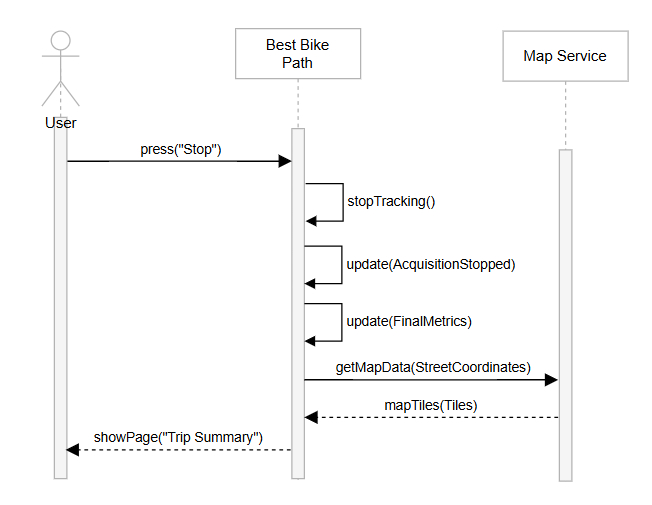
\includegraphics[width=0.8\linewidth]{RASD/Images/SEQD_stop_path_acquisition.png}
    \label{fig:placeholder}
\end{figure}
\newpage
\noindent
    \textbf{[SD15] Publish Path Automatated Mode Sequence Diagram} 
\vspace{2mm}
\begin{figure}[!h]
    \centering
    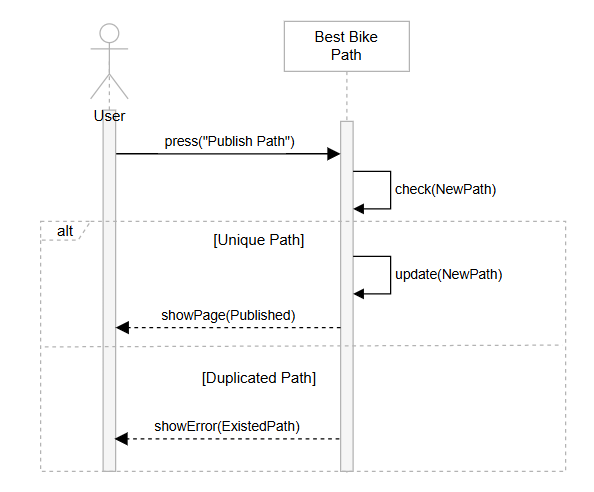
\includegraphics[width=0.8\linewidth]{RASD/Images/SEQD_publish_path_automated_mode.png}
    \label{fig:placeholder}
\end{figure}

\newpage
\subsection{Requirements Mapping}
\begin{table}[H]
    \centering
    % Aumenta lo spazio tra le righe per leggibilità
    \renewcommand{\arraystretch}{1.5}
    
    % Definizione tabella: larghezza totale testo, bordo verticale, colonna stretta per ID, colonna larga X per testo
    \begin{tabularx}{\textwidth}{|l X|}
        \hline
        % Riga Intestazione (G1) che occupa due colonne
        \multicolumn{2}{|l|}{\textbf{G1}: Registered users should have access to performance metrics about their trips.} \\
        \hline
        & \\[-1em] % Piccolo aggiustamento spaziatura
        
        % Domain Assumptions
        {[D12]} & The user’s device is equipped with a GPS, an accelerometer and a gyroscope. \\
        {[D2]} & The user has a working internet connection. \\
        {[D6]} & The external map service is available and provides accurate topographical data.\\
        & \\
        \hline
        & \\[-1em]
        
        % Requirements
        {[R1]} & The platform shall allow new users to register an account by providing personal information. \\
        {[R2]} & The platform shall allow registered users to log in by entering their registered email and password. \\
        {[R8]} & The platform shall allow users to start the navigation mode for the currently selected path. \\
        {[R12]} & When the navigation is completed, the platform shall present to registered users a summary screen
        containing statistics and the map of the path taken. \\
        {[R17]} & The platform shall display real-time metrics during the trip, including duration, current speed,
        distance traveled, and weather conditions. \\
        {[R18]} & The platform shall allow registered users to stop the recording and immediately transition to the summary screen to review the captured data. \\
        {[R25]} & The platform shall display a dashboard listing the user’s historical trips and their data, sorted chronologically.\\
        {[R29]} & The platform shall display a user profile screen summarizing the main aggregate statistics. \\
        & \\
        \hline
    \end{tabularx}
\end{table}

\newpage
\begin{table}[H]
    \centering
    % Aumenta lo spazio tra le righe per leggibilità
    \renewcommand{\arraystretch}{1.5}
    
    % Definizione tabella: larghezza totale testo, bordo verticale, colonna stretta per ID, colonna larga X per testo
    \begin{tabularx}{\textwidth}{|l X|}
        \hline
        % --- CORREZIONE QUI SOTTO ---
        % Uso 'p' con una larghezza calcolata (larghezza totale - margini interni) invece di 'l'
        % Questo obbliga il testo lungo ad andare a capo.
        \multicolumn{2}{|p{\dimexpr\textwidth-2\tabcolsep}|}{\textbf{G2}: When available, users would like to be informed about meteorological information related to the paths of interest.} \\
        \hline
        & \\[-1em] % Piccolo aggiustamento spaziatura
        
        % Domain Assumptions
        {[D2]} & The user has a working internet connection. \\
        {[D5]} & The external weather information service is reliable.\\
        & \\
        \hline
        & \\[-1em]
        
        % Requirements
        {[R1]} & The platform shall allow new users to register an account by providing personal information. \\
        {[R2]} & The platform shall allow registered users to log in by entering their registered email and password. \\
        {[R17]} & The platform shall display real-time metrics during the trip, including duration, current speed, distance traveled, and weather conditions. \\
        {[R25]} & The platform shall display a dashboard listing the user’s historical trips and their data, sorted chronologically. \\ % Corretto: rimosso '&' extra
        & \\
        \hline
    \end{tabularx}
\end{table}